\documentclass[]{article}
\usepackage{lmodern}
\usepackage{amssymb,amsmath}
\usepackage{ifxetex,ifluatex}
\usepackage{fixltx2e} % provides \textsubscript
\ifnum 0\ifxetex 1\fi\ifluatex 1\fi=0 % if pdftex
  \usepackage[T1]{fontenc}
  \usepackage[utf8]{inputenc}
\else % if luatex or xelatex
  \ifxetex
    \usepackage{mathspec}
  \else
    \usepackage{fontspec}
  \fi
  \defaultfontfeatures{Ligatures=TeX,Scale=MatchLowercase}
\fi
% use upquote if available, for straight quotes in verbatim environments
\IfFileExists{upquote.sty}{\usepackage{upquote}}{}
% use microtype if available
\IfFileExists{microtype.sty}{%
\usepackage{microtype}
\UseMicrotypeSet[protrusion]{basicmath} % disable protrusion for tt fonts
}{}
\usepackage[margin=1in]{geometry}
\usepackage{hyperref}
\hypersetup{unicode=true,
            pdftitle={Probabilidade},
            pdfauthor={Fernando B. Sabino da Silva},
            pdfborder={0 0 0},
            breaklinks=true}
\urlstyle{same}  % don't use monospace font for urls
\usepackage{color}
\usepackage{fancyvrb}
\newcommand{\VerbBar}{|}
\newcommand{\VERB}{\Verb[commandchars=\\\{\}]}
\DefineVerbatimEnvironment{Highlighting}{Verbatim}{commandchars=\\\{\}}
% Add ',fontsize=\small' for more characters per line
\usepackage{framed}
\definecolor{shadecolor}{RGB}{248,248,248}
\newenvironment{Shaded}{\begin{snugshade}}{\end{snugshade}}
\newcommand{\KeywordTok}[1]{\textcolor[rgb]{0.13,0.29,0.53}{\textbf{#1}}}
\newcommand{\DataTypeTok}[1]{\textcolor[rgb]{0.13,0.29,0.53}{#1}}
\newcommand{\DecValTok}[1]{\textcolor[rgb]{0.00,0.00,0.81}{#1}}
\newcommand{\BaseNTok}[1]{\textcolor[rgb]{0.00,0.00,0.81}{#1}}
\newcommand{\FloatTok}[1]{\textcolor[rgb]{0.00,0.00,0.81}{#1}}
\newcommand{\ConstantTok}[1]{\textcolor[rgb]{0.00,0.00,0.00}{#1}}
\newcommand{\CharTok}[1]{\textcolor[rgb]{0.31,0.60,0.02}{#1}}
\newcommand{\SpecialCharTok}[1]{\textcolor[rgb]{0.00,0.00,0.00}{#1}}
\newcommand{\StringTok}[1]{\textcolor[rgb]{0.31,0.60,0.02}{#1}}
\newcommand{\VerbatimStringTok}[1]{\textcolor[rgb]{0.31,0.60,0.02}{#1}}
\newcommand{\SpecialStringTok}[1]{\textcolor[rgb]{0.31,0.60,0.02}{#1}}
\newcommand{\ImportTok}[1]{#1}
\newcommand{\CommentTok}[1]{\textcolor[rgb]{0.56,0.35,0.01}{\textit{#1}}}
\newcommand{\DocumentationTok}[1]{\textcolor[rgb]{0.56,0.35,0.01}{\textbf{\textit{#1}}}}
\newcommand{\AnnotationTok}[1]{\textcolor[rgb]{0.56,0.35,0.01}{\textbf{\textit{#1}}}}
\newcommand{\CommentVarTok}[1]{\textcolor[rgb]{0.56,0.35,0.01}{\textbf{\textit{#1}}}}
\newcommand{\OtherTok}[1]{\textcolor[rgb]{0.56,0.35,0.01}{#1}}
\newcommand{\FunctionTok}[1]{\textcolor[rgb]{0.00,0.00,0.00}{#1}}
\newcommand{\VariableTok}[1]{\textcolor[rgb]{0.00,0.00,0.00}{#1}}
\newcommand{\ControlFlowTok}[1]{\textcolor[rgb]{0.13,0.29,0.53}{\textbf{#1}}}
\newcommand{\OperatorTok}[1]{\textcolor[rgb]{0.81,0.36,0.00}{\textbf{#1}}}
\newcommand{\BuiltInTok}[1]{#1}
\newcommand{\ExtensionTok}[1]{#1}
\newcommand{\PreprocessorTok}[1]{\textcolor[rgb]{0.56,0.35,0.01}{\textit{#1}}}
\newcommand{\AttributeTok}[1]{\textcolor[rgb]{0.77,0.63,0.00}{#1}}
\newcommand{\RegionMarkerTok}[1]{#1}
\newcommand{\InformationTok}[1]{\textcolor[rgb]{0.56,0.35,0.01}{\textbf{\textit{#1}}}}
\newcommand{\WarningTok}[1]{\textcolor[rgb]{0.56,0.35,0.01}{\textbf{\textit{#1}}}}
\newcommand{\AlertTok}[1]{\textcolor[rgb]{0.94,0.16,0.16}{#1}}
\newcommand{\ErrorTok}[1]{\textcolor[rgb]{0.64,0.00,0.00}{\textbf{#1}}}
\newcommand{\NormalTok}[1]{#1}
\usepackage{longtable,booktabs}
\usepackage{graphicx,grffile}
\makeatletter
\def\maxwidth{\ifdim\Gin@nat@width>\linewidth\linewidth\else\Gin@nat@width\fi}
\def\maxheight{\ifdim\Gin@nat@height>\textheight\textheight\else\Gin@nat@height\fi}
\makeatother
% Scale images if necessary, so that they will not overflow the page
% margins by default, and it is still possible to overwrite the defaults
% using explicit options in \includegraphics[width, height, ...]{}
\setkeys{Gin}{width=\maxwidth,height=\maxheight,keepaspectratio}
\IfFileExists{parskip.sty}{%
\usepackage{parskip}
}{% else
\setlength{\parindent}{0pt}
\setlength{\parskip}{6pt plus 2pt minus 1pt}
}
\setlength{\emergencystretch}{3em}  % prevent overfull lines
\providecommand{\tightlist}{%
  \setlength{\itemsep}{0pt}\setlength{\parskip}{0pt}}
\setcounter{secnumdepth}{5}
% Redefines (sub)paragraphs to behave more like sections
\ifx\paragraph\undefined\else
\let\oldparagraph\paragraph
\renewcommand{\paragraph}[1]{\oldparagraph{#1}\mbox{}}
\fi
\ifx\subparagraph\undefined\else
\let\oldsubparagraph\subparagraph
\renewcommand{\subparagraph}[1]{\oldsubparagraph{#1}\mbox{}}
\fi

%%% Use protect on footnotes to avoid problems with footnotes in titles
\let\rmarkdownfootnote\footnote%
\def\footnote{\protect\rmarkdownfootnote}

%%% Change title format to be more compact
\usepackage{titling}

% Create subtitle command for use in maketitle
\newcommand{\subtitle}[1]{
  \posttitle{
    \begin{center}\large#1\end{center}
    }
}

\setlength{\droptitle}{-2em}
  \title{Probabilidade}
  \pretitle{\vspace{\droptitle}\centering\huge}
  \posttitle{\par}
  \author{Fernando B. Sabino da Silva}
  \preauthor{\centering\large\emph}
  \postauthor{\par}
  \date{}
  \predate{}\postdate{}


\begin{document}
\maketitle

{
\setcounter{tocdepth}{2}
\tableofcontents
}
\section{Probabilidade de eventos}\label{probabilidade-de-eventos}

\subsection{O conceito de
probabilidade}\label{o-conceito-de-probabilidade}

\begin{itemize}
\tightlist
\item
  Experimento: Medir o tempo de espera em uma fila. Se o tempo exceder 2
  minutos marque \(1\) e 0, caso contrário.
\item
  O experimento é realizado \(n\) vezes com resultados
  \(y_1,y_2,\ldots,y_n\). Há uma \textbf{variação aleatória} no
  resultado, i.e.~às vezes ocorre \(1\) e em outras vezes ocorre 0.
\item
  \textbf{Probabilidade empírica} de exceder 2 minutos:\\
  \[ 
  p_n = \frac{\sum_{i=1}^n y_i}{n}.
  \]
\item
  \textbf{Probabilidade teórica} de exceder 2 minutos:~ \[
  p = \lim_{n\rightarrow\infty} p_n.
  \].
\item
  Tentamos inferir o verdadeiro valor de \(p\) com base em uma amostra.
  Por exemplo, ``\(p > 0.1\)?'' (``mais de \$1\$0\% dos clientes
  experimentaram um tempo de espera superior a 2 minutos?'').
\item
  A (inferência) estatística está preocupada com tais questões que são
  úteis para a tomada de decisões. Em geral, só temos acesso a uma
  amostra finita.
\end{itemize}

\subsection{Experimento real}\label{experimento-real}

\begin{itemize}
\tightlist
\item
  Em um determinado mês de 2017,~um grupo de estudantes respondeu a
  pergunta de quanto tempo eles precisaram esperar na fila em uma
  determinada cantina (em minutos):
\end{itemize}

\begin{Shaded}
\begin{Highlighting}[]
\NormalTok{y_cantina <-}\StringTok{ }\KeywordTok{c}\NormalTok{(}\DecValTok{2}\NormalTok{, }\DecValTok{5}\NormalTok{, }\DecValTok{1}\NormalTok{, }\DecValTok{6}\NormalTok{, }\DecValTok{1}\NormalTok{, }\DecValTok{1}\NormalTok{, }\DecValTok{1}\NormalTok{, }\DecValTok{1}\NormalTok{, }\DecValTok{3}\NormalTok{, }\DecValTok{4}\NormalTok{, }\DecValTok{1}\NormalTok{, }\DecValTok{2}\NormalTok{, }\DecValTok{1}\NormalTok{, }\DecValTok{2}\NormalTok{, }\DecValTok{2}\NormalTok{, }\DecValTok{2}\NormalTok{, }\DecValTok{4}\NormalTok{, }\DecValTok{2}\NormalTok{, }\DecValTok{2}\NormalTok{, }\DecValTok{5}\NormalTok{, }\DecValTok{20}\NormalTok{, }\DecValTok{2}\NormalTok{, }\DecValTok{1}\NormalTok{, }\DecValTok{1}\NormalTok{, }\DecValTok{1}\NormalTok{, }\DecValTok{1}\NormalTok{)}
\NormalTok{x_cantina <-}\StringTok{ }\KeywordTok{ifelse}\NormalTok{(y_cantina }\OperatorTok{>}\StringTok{ }\DecValTok{2}\NormalTok{, }\DecValTok{1}\NormalTok{, }\DecValTok{0}\NormalTok{)}
\NormalTok{x_cantina}
\end{Highlighting}
\end{Shaded}

\begin{verbatim}
##  [1] 0 1 0 1 0 0 0 0 1 1 0 0 0 0 0 0 1 0 0 1 1 0 0 0 0 0
\end{verbatim}

\begin{itemize}
\tightlist
\item
  Probabilidade empírica de esperar mais de 2 minutos:
\end{itemize}

\begin{Shaded}
\begin{Highlighting}[]
\NormalTok{p_cantina <-}\StringTok{ }\KeywordTok{sum}\NormalTok{(x_cantina) }\OperatorTok{/}\StringTok{ }\KeywordTok{length}\NormalTok{(x_cantina)}
\NormalTok{p_cantina}
\end{Highlighting}
\end{Shaded}

\begin{verbatim}
## [1] 0.2692308
\end{verbatim}

\begin{itemize}
\tightlist
\item
  Questão: A probabilidade na população é \(p > 1/3\)?
\item
  Nota: Um estudante disse que esperou por 20 minutos. Dado os outros
  resultados, podemos duvidar da veracidade e ignorar essa observação).
\end{itemize}

\subsection{Outro experimento}\label{outro-experimento}

\begin{itemize}
\tightlist
\item
  John Kerrich, um matemático sul-africano, estava visitando Copenhague
  quando a segunda Guerra Mundial eclodiu. Dois dias antes ele estava
  programado para viajar para a Inglaterra quando os alemães invadiram a
  Dinamarca. Kerrich passou o resto da guerra em um acampamento e para
  passar o tempo realizou uma série de experimentos. Em um destes, ele
  jogou uma moeda 10,000 vezes. Os resultados são mostrados a seguir.
\item
  Abaixo, \texttt{x} é um vetor com os primeiros 2000 resultados do
  experimento de John Kerrich. (0 = coroa,~\(1\) = cara):
\end{itemize}

\begin{Shaded}
\begin{Highlighting}[]
\KeywordTok{head}\NormalTok{(x, }\DecValTok{10}\NormalTok{)}
\end{Highlighting}
\end{Shaded}

\begin{verbatim}
##  [1] 0 0 0 1 1 1 0 1 0 0
\end{verbatim}

\begin{itemize}
\tightlist
\item
  Gráfico da probabilidade empírica \(p_n\) de sair cara contra o número
  de lançamentos \(n\):
\end{itemize}

\begin{center}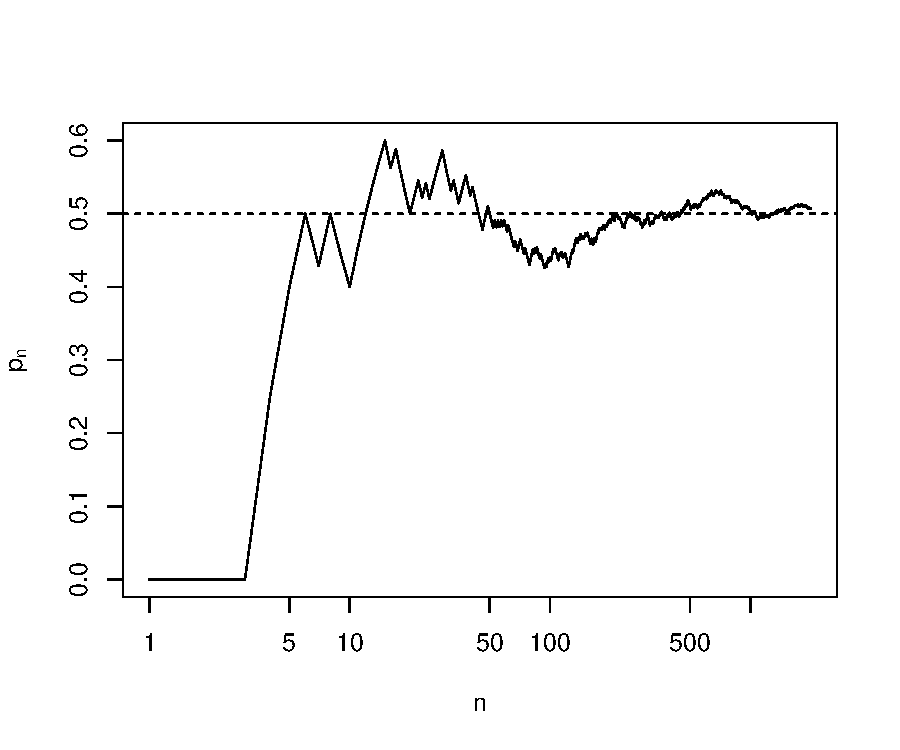
\includegraphics{probability_files/figure-latex/unnamed-chunk-7-1} \end{center}

(O eixo horizontal está na escala log).

\subsection{Definições}\label{definicoes}

\begin{itemize}
\tightlist
\item
  \textbf{Espaço Amostral}:~Todos os possíveis resultados de um
  experimento.
\item
  \textbf{Evento}:~Qualquer subconjunto do espaço amostral.
\end{itemize}

Nós conduzimos o experimento \(n\) vezes. Seja \(\#(A)\) o número de
vezes que observamos o evento \(A\).

\begin{itemize}
\tightlist
\item
  \textbf{Probabilidade empírica} do evento \(A\): \[
    p_n(A)=\frac{\#(A)}{n}.
    \]
\item
  \textbf{Probabilidade teórica} do evento \(A\): \[
    P(A)=\lim_{n\to\infty}p_n(A)
    \] 
\end{itemize}

\subsection{Probabilidades teóricas de dois
eventos}\label{probabilidades-teoricas-de-dois-eventos}

\begin{itemize}
\tightlist
\item
  Se dois eventos \(A\) e \(B\) são \textbf{disjuntos} (sem intersecção)
  então

  \begin{itemize}
  \tightlist
  \item
    \(\#(A \text{ e } B) = 0\) implica que \(P(A \cap B)=0.\)
  \item
    \(\#(A \text{ ou } B)=\#(A)+\#(B)\) implica que
    \(P(A \cup B)=P(A)+P(B).\)
  \end{itemize}
\end{itemize}

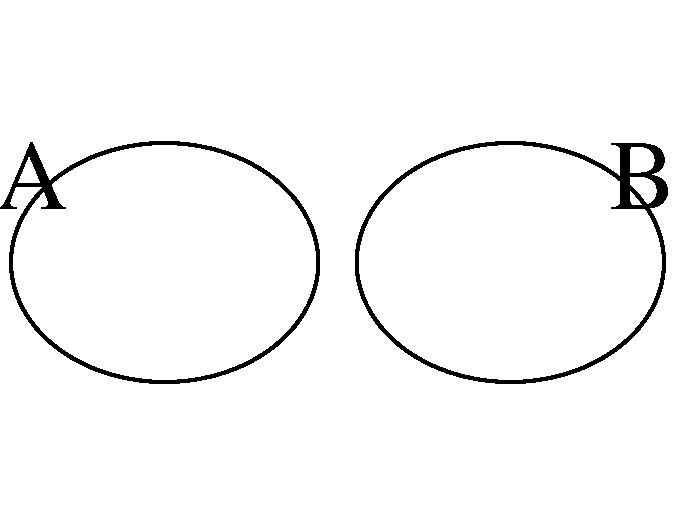
\includegraphics{probability_files/figure-latex/unnamed-chunk-8-1.pdf}

\begin{itemize}
\tightlist
\item
  Se dois eventos \(A\) e \(B\) \textbf{não são disjuntos} então a
  fórmula mais geral é \[
    P(A \cup B) = P(A) + P(B) - P(A \cap B).
    \]
\end{itemize}

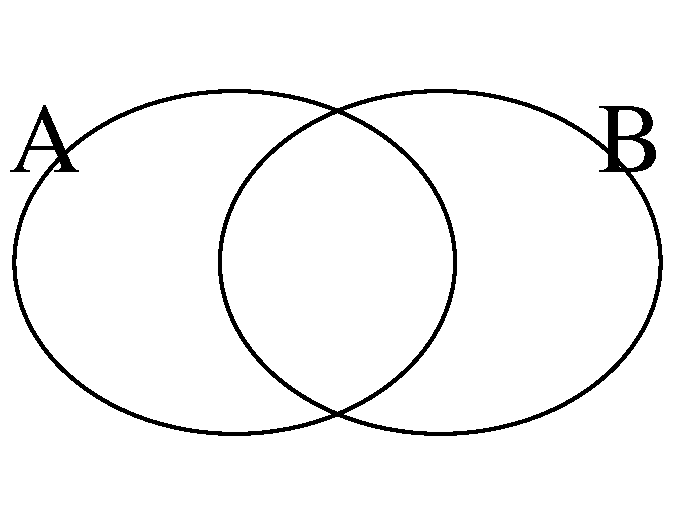
\includegraphics{probability_files/figure-latex/unnamed-chunk-9-1.pdf}

\subsection{Probabilidade Condicional}\label{probabilidade-condicional}

\begin{itemize}
\tightlist
\item
  Digamos que consideramos dois eventos \(A\) e \(B\).~Então a
  \textbf{probabilidade condicional} de \(A\) dado (ou condicional ao) o
  evento \(B\) é escrito \(P(A \mid B)\) e é definido por
  \[P(A \mid B)=\frac{P(A \cap B)}{P(B)}.\]
\item
  A probabilidade acima pode ser entendida do seguinte modo: ``quão
  provável é o evento \(A\) se nós sabemos que \(B\) ocorreu''.
\end{itemize}

\begin{center}\rule{0.5\linewidth}{\linethickness}\end{center}

\subsubsection{Exemplo com os dados das
revistas:}\label{exemplo-com-os-dados-das-revistas}

\begin{Shaded}
\begin{Highlighting}[]
\NormalTok{magAds <-}\StringTok{ }\KeywordTok{read.delim}\NormalTok{(}\StringTok{"C:/Users/fsabino/Desktop/Codes/papers/Introductory_Stat_I/notebook/datasets_ads.txt"}\NormalTok{)}

\CommentTok{# Criando dois novos fatores: 'words' e 'education':}
\NormalTok{magAds}\OperatorTok{$}\NormalTok{words <-}\StringTok{ }\KeywordTok{cut}\NormalTok{(magAds}\OperatorTok{$}\NormalTok{WDS, }\DataTypeTok{breaks =} \KeywordTok{c}\NormalTok{(}\DecValTok{31}\NormalTok{, }\DecValTok{72}\NormalTok{, }\DecValTok{146}\NormalTok{, }\DecValTok{230}\NormalTok{), }\DataTypeTok{include.lowest =} \OtherTok{TRUE}\NormalTok{)}
\NormalTok{magAds}\OperatorTok{$}\NormalTok{education <-}\StringTok{ }\KeywordTok{factor}\NormalTok{(magAds}\OperatorTok{$}\NormalTok{GROUP, }\DataTypeTok{levels =} \KeywordTok{c}\NormalTok{(}\DecValTok{1}\NormalTok{, }\DecValTok{2}\NormalTok{, }\DecValTok{3}\NormalTok{), }\DataTypeTok{labels =} \KeywordTok{c}\NormalTok{(}\StringTok{"high"}\NormalTok{, }\StringTok{"medium"}\NormalTok{, }\StringTok{"low"}\NormalTok{))}

\KeywordTok{library}\NormalTok{(mosaic)}
\end{Highlighting}
\end{Shaded}

\begin{verbatim}
## Warning: package 'mosaic' was built under R version 3.4.3
\end{verbatim}

\begin{verbatim}
## Warning: package 'dplyr' was built under R version 3.4.3
\end{verbatim}

\begin{verbatim}
## Warning: package 'ggformula' was built under R version 3.4.3
\end{verbatim}

\begin{verbatim}
## Warning: package 'ggplot2' was built under R version 3.4.3
\end{verbatim}

\begin{verbatim}
## Warning: package 'mosaicData' was built under R version 3.4.3
\end{verbatim}

\begin{verbatim}
## Warning: package 'Matrix' was built under R version 3.4.4
\end{verbatim}

\begin{Shaded}
\begin{Highlighting}[]
\NormalTok{tab <-}\StringTok{ }\KeywordTok{tally}\NormalTok{( }\OperatorTok{~}\StringTok{ }\NormalTok{words }\OperatorTok{+}\StringTok{ }\NormalTok{education, }\DataTypeTok{data =}\NormalTok{ magAds)}
\NormalTok{tab}
\end{Highlighting}
\end{Shaded}

\begin{verbatim}
##            education
## words       high medium low
##   [31,72]      4      6   5
##   (72,146]     5      6   8
##   (146,230]    9      6   5
\end{verbatim}

\begin{itemize}
\tightlist
\item
  O evento \(A\)=\(\{\)words=(146,230{]}\(\}\) (o anúncio é um texto
  ``difícil'') tem probabilidade empírica
  \[ p_n(A) = \frac{9 + 6 + 5}{54} = \frac{20}{54} \approx 37 \%.\]
\item
  Digamos que só estamos interessados na probabilidade de um texto
  ``difícil'' (evento \(A\)) para revistas de educação superior (high
  education), i.e.~condicionando no evento \(B=\{\)education=high\(\}\).
  Então a probabilidade condicional empírica pode ser calculada a partir
  da tabela acima:
\end{itemize}

\[
  p_n(A \mid B) = \frac{9}{4+5+9} = \frac{9}{18} = 0.5 = 50\%.
  \]

\begin{itemize}
\tightlist
\item
  A probabilidade condicional de \(A\) dado \(B\) pode ser
  (teoricamente) expressada por
\end{itemize}

\[
  \begin{aligned}
  P(A \mid B) 
  &= P(\text{words} =(146,230] \mid \text{education = high})  \\[0.5em]
  &= \frac{P(\text{words} =(146,230] \cap \text{education = high})}{P(\text{education = high})},  \\
  \end{aligned}
  \] que traduzindo para a probabilidade empírica (substituindo \(P\)
por \(p_n\)) dará

\[
  \begin{aligned}
  p_n(A \mid B) 
  &= \frac{p_n(\text{words} =(146,230] \cap \text{education = high})}{p_n(\text{education = high})}  \\
  &= \frac{\frac{9}{54}}{\frac{4+5+9}{54}} \\
  &= \frac{9}{4+5+9} \\[0.5em]
  &= 50\%
  \end{aligned}
  \] como calculado acima.

\subsection{Probabilidade condicional e
independência}\label{probabilidade-condicional-e-independencia}

\begin{itemize}
\tightlist
\item
  Se a informação sobre \(B\) não muda a probabilidade de \(A\) nós
  dizemos que \(A\) é \textbf{independente} de \(B\) e escrevemos \[
    P(A \mid B) = P(A) \quad \Leftrightarrow  \quad P(A \cap B) = P(A)P(B)
    \] Quando isto acontecer nós dizemos que \(A\) e \(B\) são
  \textbf{eventos independentes}.
\item
  Em geral, os eventos \(A_1, A_2, ..., A_k\) são independentes se \[
    P(A_1 \cap A_2 \cap ... \cap A_k) = P(A_1) P(A_2) \cdots P(A_k)
    \] e se o produto de todas as combinações de ordem 2 a k-1 também
  são válidas, i.e., k eventos são ditos independentes se são
  \textbf{independentes k a k, (k-1) a (k-1),\ldots{}, dois a dois},
  isto é, para cada subconjunto \(S\) de \({1, 2,\ldots k}\).
\end{itemize}

\subsubsection{Dados das revistas
revisitados}\label{dados-das-revistas-revisitados}

\begin{itemize}
\tightlist
\item
  Lembre-se das probabilidades empíricas calculadas acima: \[
  p_n(A) = 37 \%
  \quad \text{e} \quad
  p_n(A \mid B) = 50\%.
  \]
\item
  Isto indica (não podemos dizer com certeza, pois só temos a disposição
  uma amostra finita - no curso de estatística II vemos detalhes de como
  testar isso) que a probabilidade teórica
\end{itemize}

\[
P(A) \neq P(A \mid B)
\] e, portanto, que o conhecimento sobre o evento \(B\) (nível de
educação elevado) pode transmitir informações sobre a probabilidade do
evento \(A\) (o anúncio contém um texto ``difícil'').

\subsection{Um pouco mais de
formalidade}\label{um-pouco-mais-de-formalidade}

\subsubsection{Modelos de Probabilidade}\label{modelos-de-probabilidade}

Quando discutimos modelos de probabilidade, nós falamos de
\textbf{experimentos} aleatórios que produzem um dos vários
\textbf{resultados} possíveis. Um \textbf{modelo de probabilidade} que
descreve a incerteza de um experimento consiste em três elementos
(descrevemos dois abaixo):

\begin{itemize}
\tightlist
\item
  O \textbf{espaço amostral}, geralmente denominado por \(\Omega\),
  representando o conjunto que contém todos os resultados possíveis.
\item
  Uma \textbf{função de probabilidade} que atribui a um evento \(A\) um
  número não-negativo, \(P[A]\), que representa a probabilidade de que o
  evento \(A\) ocorra como resultado do experimento.
\end{itemize}

Nós chamamos de \(P[A]\) a \textbf{probabilidade} do evento \(A\). Um
evento \(A\) pode ser qualquer subconjunto do espaço amostral, não
necessariamente um único resultado possível. As leis da probabilidade
devem seguir uma série de regras, que são o resultado de um conjunto de
axiomas que introduziremos agora.

\subsection{Axiomas de Probabilidade}\label{axiomas-de-probabilidade}

Dado um espaço amostral \(\Omega\) para um experimento em particular, a
\textbf{função de probabilidade} associada ao experimento deve
satisfazer os seguintes axiomas.

\begin{itemize}
\tightlist
\item
  \emph{Não-negatividade}: \(P[A] \geq 0\) para qualquer evento
  \(A \subset\Omega\).
\item
  \emph{Normalização}: \(P[\Omega] = 1\). Ou seja, a probabilidade de
  todo o espaço é \(1\).
\item
  \emph{Aditividade}: Para eventos mutuamente exclusivos
  \(E_1, E_2,\ldots\)
  \[P\left[\bigcup_{i = 1}^{\infty} E_i\right] = \sum_{i = 1}^{\infty} P[E_i]\].
\end{itemize}

Usando estes axiomas, muitas regras adicionais de probabilidade podem
ser facilmente derivadas.

\subsection{Regras de Probabilidade}\label{regras-de-probabilidade}

\begin{itemize}
\tightlist
\item
  Dado um evento \(A\) e seu complemento, \(A^c\), ou seja, os
  resultados em \(\Omega\) que não estão em \(A\), temos a regra do
  \textbf{complementar}:
\end{itemize}

\[P[A^c] = 1 - P [A]\]

\begin{itemize}
\tightlist
\item
  Em geral, para dois eventos \(A\) e \(B\), temos a \textbf{regra da
  adição}:
\end{itemize}

\[P[A \cup B] = P[A] + P[B] - P[A \cap B]\] \emph{Exercício: Prove que
as relações acima são válidas usando os três axiomas de probabilidade.
Prove também que se} \(A\subseteq B\), \emph{então} \(P(A)\leq P(B)\).

\begin{itemize}
\tightlist
\item
  Se \(A\) e \(B\) também são \emph{disjuntos}, então temos:
\end{itemize}

\[ P[A \cup B] = P[A] + P[B] \] Se tivermos \(n\) eventos mutuamente
exclusivos, \(E_1, E_2,\ldots E_n\), então temos:

\[ P\left[\textstyle \bigcup_{i = 1}^{n} E_i \right] = \sum_{i = 1}^{n} P[E_i] \]

\subsection{Regra de Bayes}\label{regra-de-bayes}

Defina uma \textbf{partição} de um espaço amostral \(\Omega\) como um
conjunto de eventos disjuntos \(A_1, A_2, \ldots, A_n\) cuja união é o
espaço amostral \(\Omega\). Isso é

\[A_i \cap A_j = \emptyset \]

para todos \(i \neq j\) e

\[ \bigcup_{i = 1}^{n} A_i = \Omega. \]

Seja \(A_1, A_2, \ldots, A_n\) formam uma partição do espaço amostral,
onde \(P[A_i]>0\) para todo \(i\). Então para qualquer evento \(B\) com
\(P[B]>0\) temos a \textbf{Regra de Bayes}:

\[ P[A_i | B] = \frac{P[A_i] P[B | A_i]} {P[B]} = \frac{P[A_i] P[B | A_i]}{\sum_{i = 1}^{n} P[A_i] P[B | A_i]} \]

O denominador da última igualdade é freqüentemente chamado de
\textbf{lei da probabilidade total}:

\[ P[B] = \sum_{i = 1}^{n} P[A_i] P[B | A_i] \]

Dois eventos \(A\) e \(B\) são considerados \textbf{independentes} se
satisfizerem

\[ P[A \cap B] = P[A] \cdot P[B] \]

Uma coleção de eventos \(E_1, E_2, \ldots E_n\) é considerada
independente se

\[ P\left[\bigcap_{i\in S} E_i \right] = \prod_{i \in S} P[E_i] \]

para cada subconjunto \(S\) de \({1, 2,\ldots n}\).

\subsection{Regra de Bayes
(Continuação)}\label{regra-de-bayes-continuacao}

\begin{itemize}
\item
  As probabilidades dos estados da natureza são alteradas de acordo com
  as informações obtidas. Sempre que coletarmos uma amostra e ela
  contiver informações relevantes, as nossas probabilidades serão
  revisadas. Quanto maior informação, menor a incerteza.
\item
  Não sabemos qual é o \textbf{verdadeiro} estado da natureza (o que
  realmente ocorrerrá), mas temos uma avaliação das probabilidades
  (chamadas de probabilidades a priori, digamos, \(P(S_j)\)).
\item
  Queremos calcular as probabilidades revisadas, digamos,
  \(P(S_j | E_i)\), mas sabemos as \textbf{verossimilhanças}
  (likelihood, em inglês) \(P(E_i | S_j)\) = probabilidade do resultado
  experimental (\(E_i\)) condicional aos estados de natureza (\(S_j\)).
\end{itemize}

\includegraphics{C:/Users/fsabino/Desktop/Codes/papers/Introductory_Stat_I/notebook/Bayes.jpg}

\subsection{Exercício: Problema de Diagnóstico
Médico}\label{exercicio-problema-de-diagnostico-medico}

\(1\). Diagnóstico Médico: Suponha que \(1\)\% da população de um
determinado lugar seja HIV positivo. O Departamento de Saúde Pública tem
um teste de diagnóstico barato que é administrado às pessoas que pedem
para serem testadas. O teste resulta em uma indicação positiva ou
negativa e apresenta as seguintes características:

\begin{enumerate}
\def\labelenumi{(\alph{enumi})}
\item
  O teste dá uma indicação positiva (verdadeira) 99\% das vezes em que
  uma pessoa é realmente portadora do vírus. Infelizmente, o teste dá
  uma indicação negativa (falsa) para \(1\)\% das pessoas que portam o
  vírus.
\item
  O teste dá uma indicação negativa (verdadeira) 95\% das vezes em que
  uma pessoa não é portadora do vírus (e, portanto, dá uma indicação
  positiva (falsa) para 5\% das pessoas).
\end{enumerate}

\begin{itemize}
\item
  Suponha que um residente escolhido ao acaso tenha acabado de fazer o
  teste. Para seu choque, o teste resultou em uma indicação positiva.
  Qual é a probabilidade dele ser realmente portador do vírus?
\item
  Suponha agora que o teste tenha resultado em uma indicação negativa. O
  residente deve ficar confiante de que ele não é realmente HIV
  positivo?
\item
  Como as suas respostas mudam se o teste se tornar \(10\) vezes mais
  confiável, isto é, se as taxas de erro para falsos negativos e falsos
  positivos, respectivamente, forem reduzidas para \(0.1\)\% e 0.5\%?
\end{itemize}

\subsection{Exercício: Problema de Controle de
Qualidade}\label{exercicio-problema-de-controle-de-qualidade}

\(2\). Controle de Qualidade: A DataSafe produz pen drives. Seu processo
de fabricação é direcionado para produzir defeitos a uma taxa de
\(1/10\) de \(1\)\%, isto é, \(0.1\)\%. Às vezes, quando o processo é
iniciado, ele desliza ligeiramente e produz defeitos a uma taxa de
\(2/10\) de \(1\)\%. Como parar o maquinário para recalibrar o processo
é muito caro, a DataSafe está disposta a operar com uma taxa de defeitos
um pouco maior. Ocasionalmente, no entanto, o processo se desvia tanto
que produz defeitos a uma taxa de \(5/10\) de \(1\)\%, o que é
inaceitável para a gerência. Com base em experiências passadas, o
engenheiro chefe da DataSafe, observou que, em qualquer dia, as
probabilidades para a verdadeira taxa de defeitos são:

\begin{longtable}[]{@{}lccc@{}}
\toprule
Condição Operacional & Boa & Ok & Ruim\tabularnewline
\midrule
\endhead
Taxa de Defeito & \(.001\) & \(.002\) & \(.005\)\tabularnewline
Probabilidade & \(.75\) & \(.24\) & \(.01\)\tabularnewline
\bottomrule
\end{longtable}

\begin{itemize}
\item
  No início de cada dia, ele retira uma amostra da produção inicial para
  deciri se a máquina precisa ser recalibrada. A sua regra operacional é
  recalibrar sempre que ele não puder ter pelo menos 90\% de certeza de
  que a taxa de defeitos está abaixo de \(5/10\) de \(1\)\%.
\item
  Suponha que o primeiro pen drive escolhido aleatoriamente esteja com
  defeito. A produção deveria ser parada para recalibração? E se os dois
  primeiros escolhidos aleatoriamente estiverem com defeito?
\end{itemize}

\subsection{Solução para o problema do diagnóstico
médico}\label{solucao-para-o-problema-do-diagnostico-medico}

Dada uma indicação positiva:

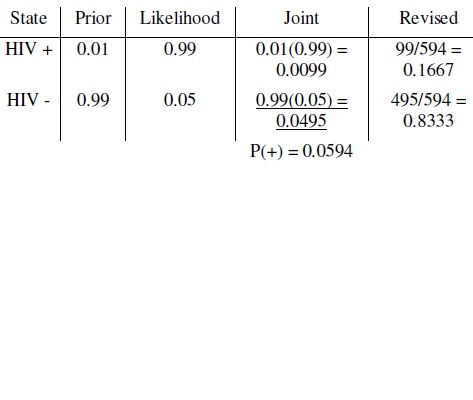
\includegraphics{C:/Users/fsabino/Desktop/Codes/papers/Introductory_Stat_I/notebook/hiv+.jpg}

Dada uma indicação negativa:

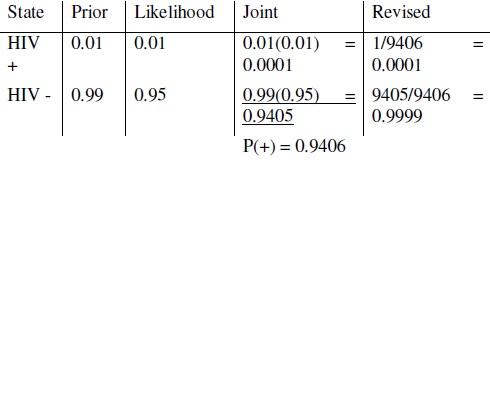
\includegraphics{C:/Users/fsabino/Desktop/Codes/papers/Introductory_Stat_I/notebook/hiv-.jpg}

\begin{itemize}
\tightlist
\item
  Se o teste se tornar \(10\) vezes mais confiável.
\end{itemize}

Dada uma indicação positiva:

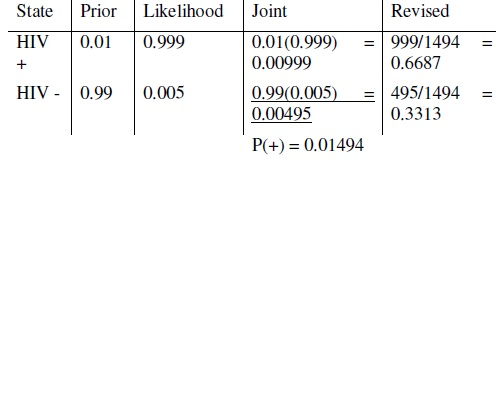
\includegraphics{C:/Users/fsabino/Desktop/Codes/papers/Introductory_Stat_I/notebook/hiv+10.jpg}

Dada uma indicação negativa:

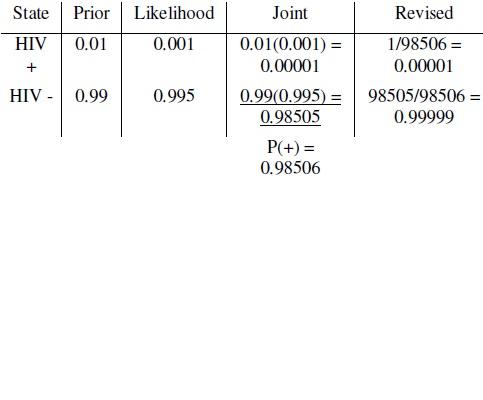
\includegraphics{C:/Users/fsabino/Desktop/Codes/papers/Introductory_Stat_I/notebook/hiv-10.jpg}

\subsection{Solução para o Problema de Controle de
Qualidade}\label{solucao-para-o-problema-de-controle-de-qualidade}

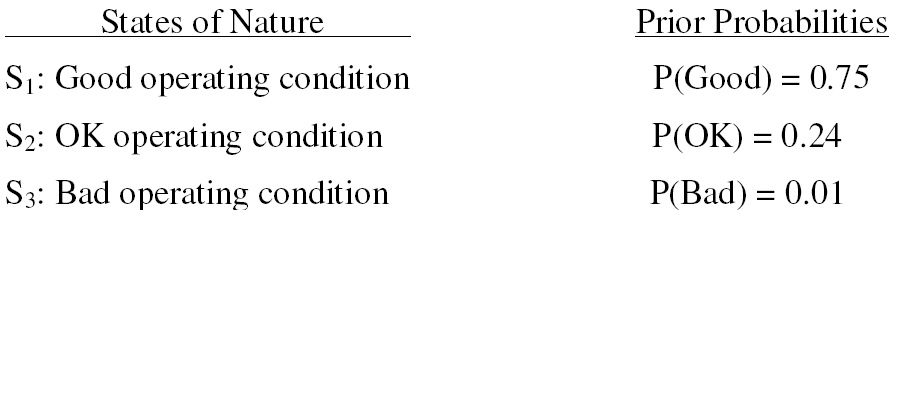
\includegraphics{C:/Users/fsabino/Desktop/Codes/papers/Introductory_Stat_I/notebook/QC1.jpg}
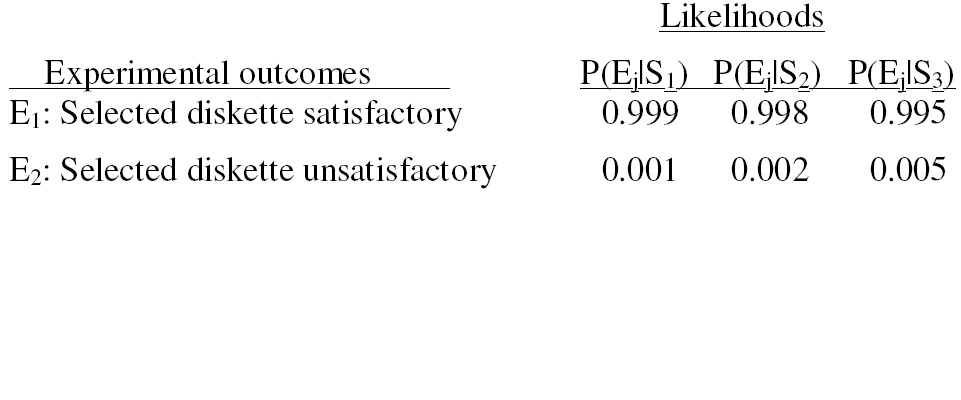
\includegraphics{C:/Users/fsabino/Desktop/Codes/papers/Introductory_Stat_I/notebook/QC2.jpg}

\begin{itemize}
\tightlist
\item
  Probabilidades revisadas dado que um pen drive defeituoso é
  selecionado:
\end{itemize}

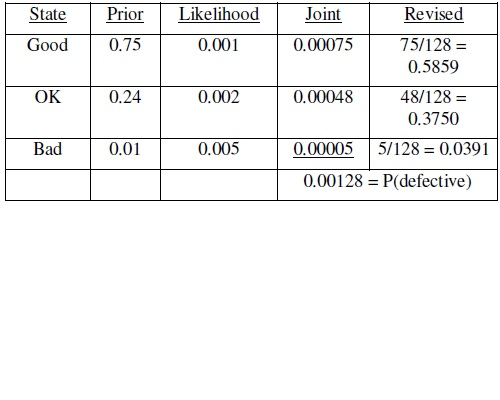
\includegraphics{C:/Users/fsabino/Desktop/Codes/papers/Introductory_Stat_I/notebook/revised.jpg}

\begin{itemize}
\item
  Então, P(Bom ou OK \textbar{} defeituoso) = 0.9609 \textgreater{} 0.9.
  Ele não deve recalibrar.
\item
  Note as implicações disso. Se o pen drive escolhido for defeituoso,
  ele não vai recalibrar. E se não estiver com defeito, ele certamente
  não irá recalibrar. Logo, amostrar apenas um pen drive é sem
  utilidade.
\item
  Probabilidades revisadas dado que dois pen drives defeituosos são
  selecionados:
\end{itemize}

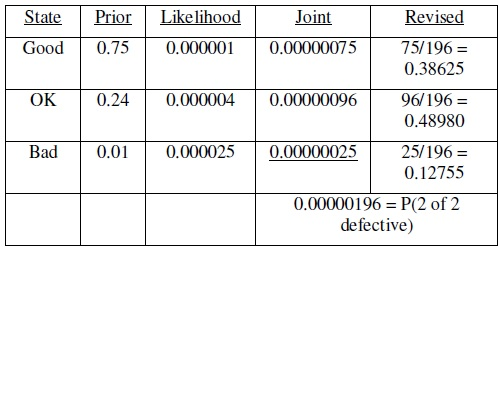
\includegraphics{C:/Users/fsabino/Desktop/Codes/papers/Introductory_Stat_I/notebook/revised2.jpg}

\begin{itemize}
\item
  Então, P(Bom ou OK \textbar{} 2 de 2 defeituosos) = 0.87245
  \textless{} 0.9. Ele deve recalibrar.
\item
  Deixo para você verificar que ele não irá recalibrar se nenhum pen
  drive amostrado estiver com defeito (seja calculando ou inferindo
  pelos que encontramos na parte anterior) ou se apenas um dos dois
  estiver com defeito.
\end{itemize}

\subsection{Distribuição discreta}\label{distribuicao-discreta}

\subsubsection{Exemplo: Dados das
revistas}\label{exemplo-dados-das-revistas}

\begin{Shaded}
\begin{Highlighting}[]
\CommentTok{# Tabela contendo o percentual de anúncios em cada combinação dos níveis de 'words' e 'education'}
\NormalTok{tab <-}\StringTok{ }\KeywordTok{tally}\NormalTok{( }\OperatorTok{~}\StringTok{ }\NormalTok{words }\OperatorTok{+}\StringTok{ }\NormalTok{education, }\DataTypeTok{data =}\NormalTok{ magAds, }\DataTypeTok{format =} \StringTok{"percent"}\NormalTok{)}
\KeywordTok{round}\NormalTok{(tab, }\DecValTok{2}\NormalTok{) }\CommentTok{# Duas casas decimais}
\end{Highlighting}
\end{Shaded}

\begin{verbatim}
##            education
## words        high medium   low
##   [31,72]    7.41  11.11  9.26
##   (72,146]   9.26  11.11 14.81
##   (146,230] 16.67  11.11  9.26
\end{verbatim}

\begin{itemize}
\tightlist
\item
  Os 9 eventos disjuntos acima (correspondentes as combinações de
  \texttt{words} e \texttt{education}) compõem todo o espaço amostral
  para as duas variáveis. As probabilidades empíricas de cada evento são
  dadas na tabela.
\end{itemize}

\subsubsection{Distribuição discreta}\label{distribuicao-discreta-1}

\begin{itemize}
\tightlist
\item
  Em geral:

  \begin{itemize}
  \tightlist
  \item
    Seja \(A_1,A_2,\ldots,A_k\) uma subdivisão do espaço amostral em
    eventos disjuntos (par a par).
  \item
    As probabilidades \(P(A_1), P(A_2), ..., P(A_k)\)
    (\textbf{distribuição discreta}) satisfazem
    \[\sum_{i=1}^kP(A_i)=1.\]
  \end{itemize}
\end{itemize}

\begin{center}\rule{0.5\linewidth}{\linethickness}\end{center}

\subsubsection{Exemplo: Três lançamentos de uma
moeda}\label{exemplo-tres-lancamentos-de-uma-moeda}

\begin{itemize}
\tightlist
\item
  \textbf{Variável aleatória}: Uma variável aleatória é simplesmente uma
  função \(Y\) que mapeia os resultados do espaço amostral para números
  reais, isto é, que mapeia os possíveis resultados do experimento em um
  número.
\item
  Resultados possíveis de um experimento com 3 lançamentos de moedas:

  \begin{itemize}
  \tightlist
  \item
    \(0\) caras (KKK)
  \item
    \(1\) cara (CKK, KCK, KKC)
  \item
    \(2\) caras (CCK, CKC, KCC)
  \item
    \(3\) caras (CCC)
  \end{itemize}
\item
  Os eventos acima são disjuntos e compõem todo o espaço amostral.
\item
  Seja \(Y\) o número de caras no experimento:
  \(Y(KKK) = 0, Y(CKK) = 1, \ldots\)
\item
  Assuma que cada resultado é igualmente provável, i.e. \(1/8\) de
  probabilidade para cada um deles. Então,

  \begin{itemize}
  \tightlist
  \item
    \(P(\text{nenhuma cara}) = P(Y = 0) = P(KKK) = 1/8.\)
  \item
    \(P(\text{uma cara}) = P(Y = 1) = P(CKK \text{ ou } KCK \text{ ou } KKC) = P(CKK) + P(KCK) + P(KKC) = 3/8.\)
  \item
    Similarmente para 2 ou 3 caras.
  \end{itemize}
\item
  Então, a distribuição de \(Y\) é
\end{itemize}

\begin{longtable}[]{@{}lrlll@{}}
\toprule
Número de caras, \(Y\) & \(0\) & \(1\) & \(2\) & \(3\)\tabularnewline
\midrule
\endhead
Probabilidade & \(1/8\) & 3/8 & 3/8 & \(1/8\)\tabularnewline
\bottomrule
\end{longtable}

\section{Distribuição de variáveis
aleatórias}\label{distribuicao-de-variaveis-aleatorias}

\subsection{Distribuição de
probabilidade}\label{distribuicao-de-probabilidade}

\begin{itemize}
\item
  Exemplo: Conduzimos um experimento no qual fazemos uma medição
  quantitativa \(Y\) (uma variável aleatória), por exemplo, contamos o
  número de palavras em um anúncio ou o tempo de espera em uma fila.
\item
  De antemão, há muitos resultados possíveis para os experimentos,
  i.e.~os valores de \(Y\) que irão acontecer em uma realização do
  experimento são incertos, mas nós podemos quantificá-los pela
  \textbf{distribuição de probabilidade} de \(Y\).
\item
  Uma definição não rigorosa, mas útil para transmitir a ideia é:
  \[ \text{distribuição} = \text{lista de possíveis} \textbf{ valores} + \text{probabilidades} \textbf{ associadas} \]
\item
  Para qualquer intervalo \((a, b\)), a distribuição indica a
  probabilidade de observar um valor da variável aleatória \(Y\) neste
  intervalo: \[ P(a<Y<b),\qquad -\infty < a < b < \infty.\]
\item
  Se os possíveis valores de uma variável aleatória são discretos, isto
  é, se nós podemos enumerar todos os possíveis valores de \(Y\), então
  a variável aleatória \(Y\) é chamada de \textbf{discreta}. Por
  exemplo, o número de palavras em um anúncio.
\item
  Se os possíveis valores de uma variável aleatória são contínuos, isto
  é, \(Y\) pode assumir qualquer valor dentro de um intervalo, então a
  variável aleatória \(Y\) é chamada de \textbf{contínua}. Por exemplo,
  o tempo de espera em uma fila.
\end{itemize}

\subsection{Variáveis Aleatórias
Discretas}\label{variaveis-aleatorias-discretas}

\begin{itemize}
\tightlist
\item
  A distribuição de uma variável aleatória discreta \(X\) é mais
  frequentemente especificada por uma lista de possíveis valores e uma
  função massa de probabilidade \(p(x)\), isto é,
\end{itemize}

\[ p(x) = p_X(x) = P[X = x]. \] Costumeiramente nós abandonamos o
subscrito da notação mais correta \(p_X(x)\) e simplesmente escrevemos
\(p(x)\). A variável aleatória relevante será discernida do contexto.

O exemplo mais comum de uma variável aleatória discreta é a variável
aleatória com distribuição binomial. A função massa de uma variável
aleatória \(X\) com distribuição binomial é dada por

\[ P(X = x | n, p) = p_X(x | n, p) = {n \choose x} p^x(1 - p)^{n - x}, \ \ \ x = 0, 1, \ldots, n, \ n \in \mathbb{N}, \ 0 < p < 1. \]

A última linha contém uma grande quantidade de informação.

\begin{itemize}
\item
  A função \(p_X(x | n, p)\) é a função massa. É uma função de \(x\), os
  possíveis valores da variável aleatória \(X\). Ela é condicional aos
  parâmetros \(n\) e \(p\). Valores diferentes destes parâmetros
  especificam distribuições binomiais diferentes.
\item
  \(x = 0, 1, \ldots, n\) indica o espaço amostral de \(x\), isto é, os
  possíveis valores da variável aleatória.
\end{itemize}

\(n \in \mathbb{N}\) e \(0 < p < 1\) especificam os espaços dos
parâmetros. Estes são os valores possíveis dos parâmetros que fornecem
uma distribuição binomial válida. Frequentemente, toda essa informação é
simplesmente codificada escrevendo

\[ X \sim \text{Bin}(n, p). \]

\subsection{Variáveis Aleatórias
Contínuas}\label{variaveis-aleatorias-continuas}

\begin{itemize}
\item
  A distribuição de uma variável aleatória contínua \(X\) é mais
  frequentemente especificada pelo conjunto de possíveis valores e uma
  função densidade de probabilidade, \(f(x)\). (A função de distribuição
  acumulada (densidade acumulada), \(F(x)\) ou a função característica
  ou geratriz de momentos também seriam suficientes.)
\item
  A probabilidade do evento \(a < X < b\) é calculada por
\end{itemize}

\[ P[a < X < b] = \int_{a}^{b} f(x)dx. \]

Note que as densidades não são probabilidades.

\begin{itemize}
\tightlist
\item
  O exemplo mais comum de uma variável aleatória contínua é uma variável
  aleatória com distribuição normal. A densidade de uma variável
  aleatória normal \(X\), é dada por
\end{itemize}

\[ f(x | \mu, \sigma^2) = \frac{1}{\sigma\sqrt{2p}} \cdot \exp\left[\frac{-1}{2} \left(\frac{x - \mu}{\sigma}\right)^2 \right], \ \ \ -\infty < x < \infty, \ -\infty < \mu < \infty, \ \sigma > 0. \]

\begin{itemize}
\tightlist
\item
  A função \(f(x | \mu, \sigma^2)\) é a função de densidade. É uma
  função de \(x\), os valores possíveis da variável aleatória \(X\). Ela
  é condicional aos parâmetros \(\mu\) e \(\sigma^2\). Diferentes
  valores destes parâmetros especificam diferentes distribuições normal.
\item
  \(-\infty < x < \infty\) indica o espaço amostral de \(x\). Neste
  caso, a variável aleatória pode assumir todo e qualquer valor real.
\item
  \(-\infty < \mu < \infty\) and \(\sigma > 0\) especificam o espaço de
  parâmetros. Estes são os valores possíveis dos parâmetros que fornecem
  uma distriuição normal válida. Muitas vezes, toda essa informação é
  simplesmente codificada escrevendo
\end{itemize}

\[ X \sim N(\mu, \sigma^2) \]

\subsection{Independência entre Variáveis
Aleatórias}\label{independencia-entre-variaveis-aleatorias}

Considere duas variáveis aleatórias \(X\) e \(Y\). Nós dizemos que elas
são independentes se

\[ f(x, y) = f(x) \cdot f(y) \]

para todo \(x\) e \(y\). Aqui \(f(x, y)\) é a função densidade (massa)
conjunta de \(X\) e \(Y\). Nós chamamos de \(f(x)\) e de \(f(y)\) as
funções densidade (massa) marginais de \(X\) e de \(Y\),
respectivamente.

\begin{itemize}
\tightlist
\item
  A função densidade (massa) conjunta \(f(x, y)\) juntamente com os
  possíveis valores \((x, y)\) especificam a distribuição conjunta de
  \(X\) e \(Y\).
\end{itemize}

Noções similares existem para mais de duas variáveis aleatórias.

\subsubsection{Amostra Aleatória}\label{amostra-aleatoria}

Nós realizamos um experimento \(n\) vezes, onde o resultado do
\(i\)-ésimo experimento corresponde a uma medição de uma variável
aleatória \(Y_i\), onde assumimos que

\begin{itemize}
\tightlist
\item
  Os experimentos são \textbf{independentes}
\item
  As variáveis \(Y_1,\ldots,Y_n\) têm a \textbf{mesma distribuição}
\end{itemize}

\subsection{Parâmetros populacionais}\label{parametros-populacionais}

\begin{itemize}
\tightlist
\item
  Quando o tamanho da amostra aumenta, a média da amostra,
  \(\overline{y}\), por exemplo, irá se estabilizar em torno de um valor
  fixo, \(\mu\), que é usualmente desconhecido. O valor \(\mu\) é
  chamado de \textbf{média populacional}.
\item
  Correspondentemente, o desvio padrão da amostra, \(s\), irá se
  estabilizar em torno de um valor fixo, \(\sigma\), que geralmente é
  desconhecido. O valor \(\sigma\) é chamado de \textbf{desvio padrão da
  população}.
\item
  Notação:

  \begin{itemize}
  \tightlist
  \item
    \(\mu\) (mu) denota a médida da população.
  \item
    \(\sigma\) (sigma) denota o desvio padrão da população.
  \end{itemize}
\end{itemize}

\begin{longtable}[]{@{}cc@{}}
\toprule
População & Amostra\tabularnewline
\midrule
\endhead
\(\mu\) & \(\overline{y}\)\tabularnewline
\(\sigma\) & \(s\)\tabularnewline
\bottomrule
\end{longtable}

\begin{center}\rule{0.5\linewidth}{\linethickness}\end{center}

\subsubsection{Distribuição de uma variável aleatória
discreta}\label{distribuicao-de-uma-variavel-aleatoria-discreta}

\begin{itemize}
\tightlist
\item
  Valores possíveis para \(Y\):~\(\{y_1,y_2,\ldots,y_k\}\).
\item
  A \textbf{distribuição} de \(Y\) é a probabilidade de cada valor
  possível:~\(p_i=P(Y=y_i), \quad i=1,2,\ldots,k\).
\item
  A distribuição satisfaz: \(\sum_{i=1}^kp_i=1\).
\end{itemize}

\subsection{Esperança}\label{esperanca}

Para variáveis aleatórias discretas, nós definimos a \textbf{esperança}
da função de uma variável aleatória \(X\) da seguinte maneira.

\[ \mathbb{E}[g(X)] \triangleq \sum_{x} g(x)p(x) \]

Para variáveis aleatórias contínuas, nós temos uma definição semelhante.

\[ \mathbb{E}[g(X)] \triangleq \int g(x)f(x) dx \]

Para funções específicas \(g\), as esperanças recebem nomes

A \textbf{média} de uma variável aleatória \(X\) é dada por

\[ \mu_{X} = \mathbb{E}[X]. \]

Então, para uma variável aleatória discreta, nós temos

\[ \text{E}[X] = \sum_{x} x \cdot p(x) \]

Para uma variável aleatória contínua, simplesmente substituímos a soma
por uma integral.

A variância de uma variável aleatória \(X\) é dada por

\[ \sigma^2_{X} = \text{var}[X] \triangleq \mathbb{E}[(X - \mathbb{E}[X])^2] = \mathbb{E}[X^2] - (\mathbb{E}[X])^2. \]

O desvio padrão de uma variável aleatória \(X\) é dada por

\[ \sigma_{X} = \text{sd}[X] \triangleq \sqrt{\sigma^2_{X}} = \sqrt{\text{var}[X]}. \]

A covariância de variáveis aleatórias \(X\) e \(Y\) é dada por

\[ \text{cov}[X, Y] \triangleq \mathbb{E}[(X - \mathbb{E}[X])(Y - \mathbb{E}[Y])] = \mathbb{E}[XY] - \mathbb{E}[X] \cdot \mathbb{E}[Y]. \]

\subsection{Verossimilhança
(Likelihood)}\label{verossimilhanca-likelihood}

Considere \(n\) variáveis aleatórias iid \(X_1, X_2, \ldots X_n\). Nós
definimos a função de verossimilhança por

\[ \mathcal{L}(\theta \mid x_1, x_2, \ldots x_n) = \prod_{i = i}^n f(x_i; \theta) \]

onde \(f(x_i; \theta)\) é a função densidade (ou massa) da variável
aleatória \(X_i\) avaliada em \(x_i\) com parâmetro \(\theta\).

Enquanto a probabilidade é uma função de um possível valor (ou
intervalo) observado, dados determinados valores dos parâmetros, a
verossimilhança é o ``oposto'': é uma função dos valores possíveis dos
parâmetros dada a amostra, i.e., verossimilhança é uma medida da
evidência que uma amostra fornece para valores específicos dos
parâmetros em um modelo paramétrico.

A maximização da verossimilhança é uma técnica comum para ajustar um
modelo aos dados.

\subsection{Valor esperado (média) para uma distribuição
discreta}\label{valor-esperado-media-para-uma-distribuicao-discreta}

\begin{itemize}
\tightlist
\item
  O \textbf{valor esperado} ou \textbf{média (populacional)} de \(Y\) é
  \[
    \mu = \sum_{i=1}^k p_iy_i
    \]
\item
  Uma propriedade importante do valor esperado é que ele tem a mesma
  unidade de medida das observações (por exemplo, metro).
\end{itemize}

\subsubsection{Exemplo: número de caras em 3 lançamentos de uma
moeda}\label{exemplo-numero-de-caras-em-3-lancamentos-de-uma-moeda}

\begin{itemize}
\item
  Lembre-se da distribuição de \(Y\) (número de caras):

  \begin{longtable}[]{@{}lcccc@{}}
  \toprule
  y (número de caras) & 0 & \(1\) & 2 & 3\tabularnewline
  \midrule
  \endhead
  \(P(Y = y)\) & \(1/8\) & 3/8 & 3/8 & \(1/8\)\tabularnewline
  \bottomrule
  \end{longtable}
\item
  Então o valor esperado é
\end{itemize}

\[
  \mu = 0\frac{1}{8}+1\frac{3}{8}+2\frac{3}{8}+3\frac{1}{8}=1.5.
  \]

\emph{Observe que o valor esperado não precisa ser um resultado possível
do próprio experimento.}

\subsection{Variância e desvio padrão de uma distribuição
discreta}\label{variancia-e-desvio-padrao-de-uma-distribuicao-discreta}

\begin{itemize}
\tightlist
\item
  A \textbf{variância (populacional)} de \(Y\) é \[
      \sigma^2 = \sum_{i=1}^k (y_i - \mu)^2 p_i
  \]
\item
  O \textbf{desvio padrão (populacional)} é
  \(\sigma = \sqrt{\sigma^2}\).
\item
  Nota: Se as observações forem medidas em metro, a \textbf{variância}
  terá unidade \(\text{metro}^2\) o que comumente não estamos
  acostumados a interpretar. O \textbf{desvio padrão}, por outro lado,
  tem a mesma unidade de medida que as observações.
\end{itemize}

\subsubsection{Exemplo: número de caras em 3 lançamentos de uma
moeda}\label{exemplo-numero-de-caras-em-3-lancamentos-de-uma-moeda-1}

A distribuição da variável aleatória `número de caras em 3 lançamentos
de uma moeda' tem variância \[ \sigma^2
    = (0-1.5)^2\frac{1}{8} + (1-1.5)^2\frac{3}{8} + (2-1.5)^2 \frac{3}{8} + (3-1.5)^2 \frac{1}{8} = 0.75.
    \]

e desvio padrão \[  \sigma = \sqrt{\sigma^2} = \sqrt{0.75} = 0.866.  \]

\subsection{A distribuição binomial}\label{a-distribuicao-binomial}

\begin{itemize}
\tightlist
\item
  A \textbf{distribuição binomial} é uma distribuição discreta.
\item
  Seja \(Y\) a variável aleatória que representa o número de sucessos
  obtidos em \(n\) experimentos aleatórios (independentes). Assuma que
  cada experimento tem apenas dois resultados possíveis, denominados
  \textbf{sucesso} e \textbf{fracasso} e que cada experimento tem a
  mesma probabilidade \(p\) de sucesso.
\item
  Dizemos que \(Y\) tem uma \textbf{distribuição binomial} com
  parâmetros \(n\) e \(p\).\\
\item
  Neste caso, podemos mostrar que
  \[p_Y(y) = P(Y = y) = \binom{n}{y} p^y (1-p)^{n-y},\] onde
  \(\binom{n}{y}=\frac{n!}{y!(n-y)!}\) e \(m!\) é o produto dos
  primeiros \(m\) inteiros.
\item
  Valor esperado: \(\mu = n p\).
\item
  Variância: \(\sigma^2 = n p (1-p)\).
\item
  Desvio padrão: \(\sigma = \sqrt{n p (1-p)}\).
\end{itemize}

\begin{Shaded}
\begin{Highlighting}[]
\CommentTok{# A distribuição binomial com n = 10 e p = 0.35:}
\KeywordTok{plotDist}\NormalTok{(}\StringTok{"binom"}\NormalTok{, }\DataTypeTok{size =} \DecValTok{10}\NormalTok{, }\DataTypeTok{prob =} \FloatTok{0.35}\NormalTok{,}
         \DataTypeTok{ylab =} \StringTok{"Probabilidade"}\NormalTok{, }\DataTypeTok{xlab =} \StringTok{"Número de sucessos"}\NormalTok{, }\DataTypeTok{main =} \StringTok{"binom(n = 10, prob = 0.35)"}\NormalTok{)}
\end{Highlighting}
\end{Shaded}

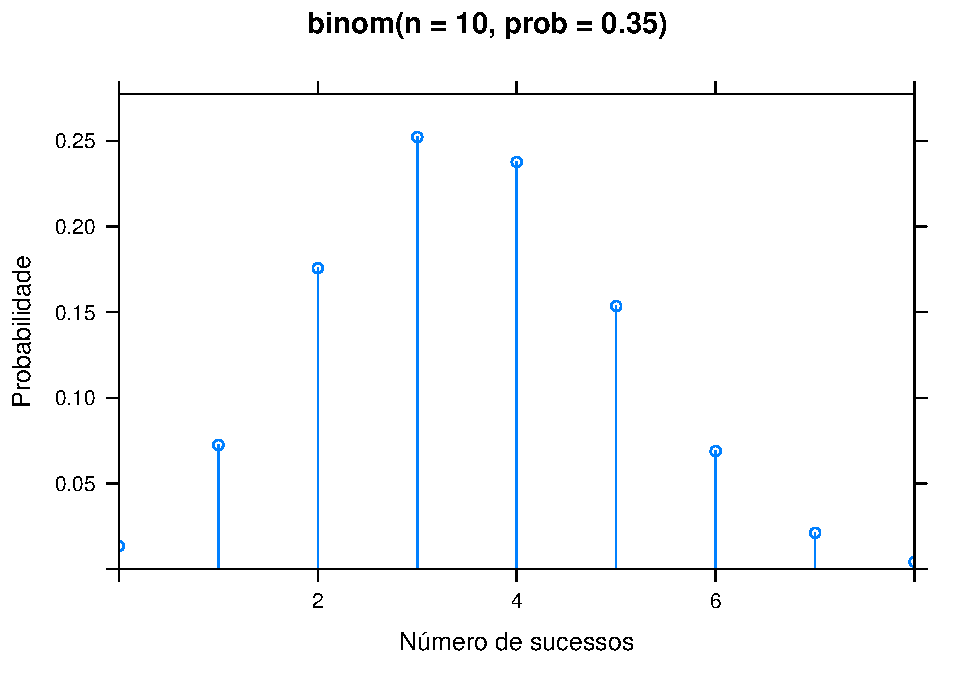
\includegraphics{probability_files/figure-latex/dbinom-1.pdf}

\subsection{Distribuição de uma variável aleatória
contínua}\label{distribuicao-de-uma-variavel-aleatoria-continua}

\begin{itemize}
\tightlist
\item
  A distribuição de uma variável aleatória contínua \(Y\) é
  caracterizada pela função densidade de probabilidade \(f_Y\).
\end{itemize}

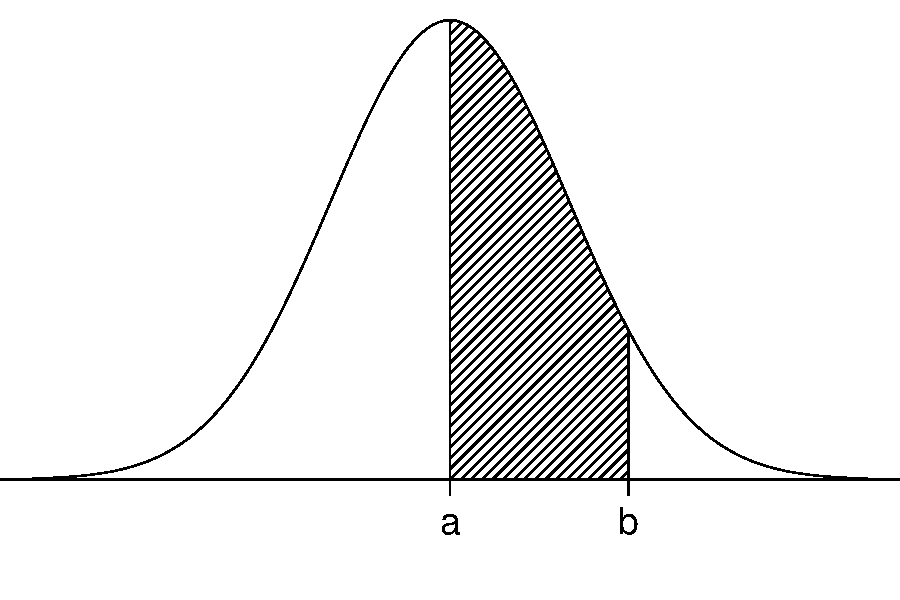
\includegraphics{probability_files/figure-latex/normprobs-1.pdf}

\begin{itemize}
\tightlist
\item
  A área sob o gráfico da função densidade de probabilidade entre \(a\)
  e \(b\) é igual a probabilidade de uma observação neste intervalo.
\item
  \(f_Y(y)\geq 0\) para todos os números reais \(y\).
\item
  A área sob o gráfico de \(f_Y\) é igual a 1.
\item
  Por exemplo, a \textbf{distribuição uniforme} de \(a\) até \(b\): \[
  f_Y(y)=
  \begin{cases}
    \frac{1}{b-a} & a<y<b \\
    0 & \text{otherwise}
  \end{cases}
  \] 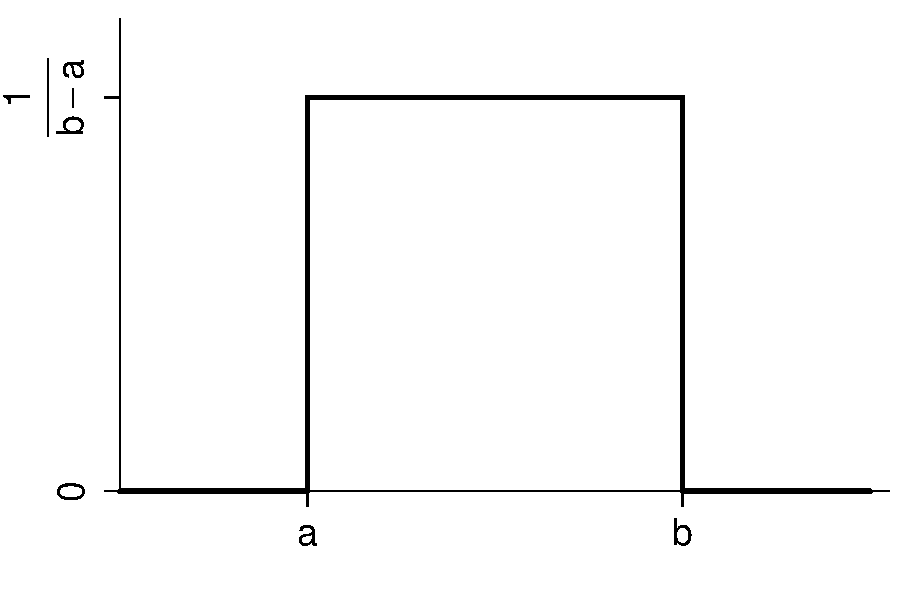
\includegraphics{probability_files/figure-latex/unifdist-1.pdf}
\end{itemize}

\subsection{Função Densidade}\label{funcao-densidade}

\subsubsection{Aumentando o número de
observações}\label{aumentando-o-numero-de-observacoes}

\begin{itemize}
\tightlist
\item
  Outra maneira de pensar sobre a densidade é em termos do histograma.
\item
  Se desenharmos um histograma para uma amostra onde a área de cada
  caixa corresponde a frequência relativa de cada intervalo, a área
  total será \(1\).
\item
  Quando o número de observações (tamanho da amostra) aumenta nós
  podemos fazer intervalos menores e obter um histograma mais suave.
\item
  Com um número infinito de observações, nós poderíamos produzir uma
  curva suave, onde a área embaixo dela é \(1\).~Uma função derivada
  dessa forma é o que nós chamamos de \textbf{função densidade de
  probabilidade}.
\end{itemize}

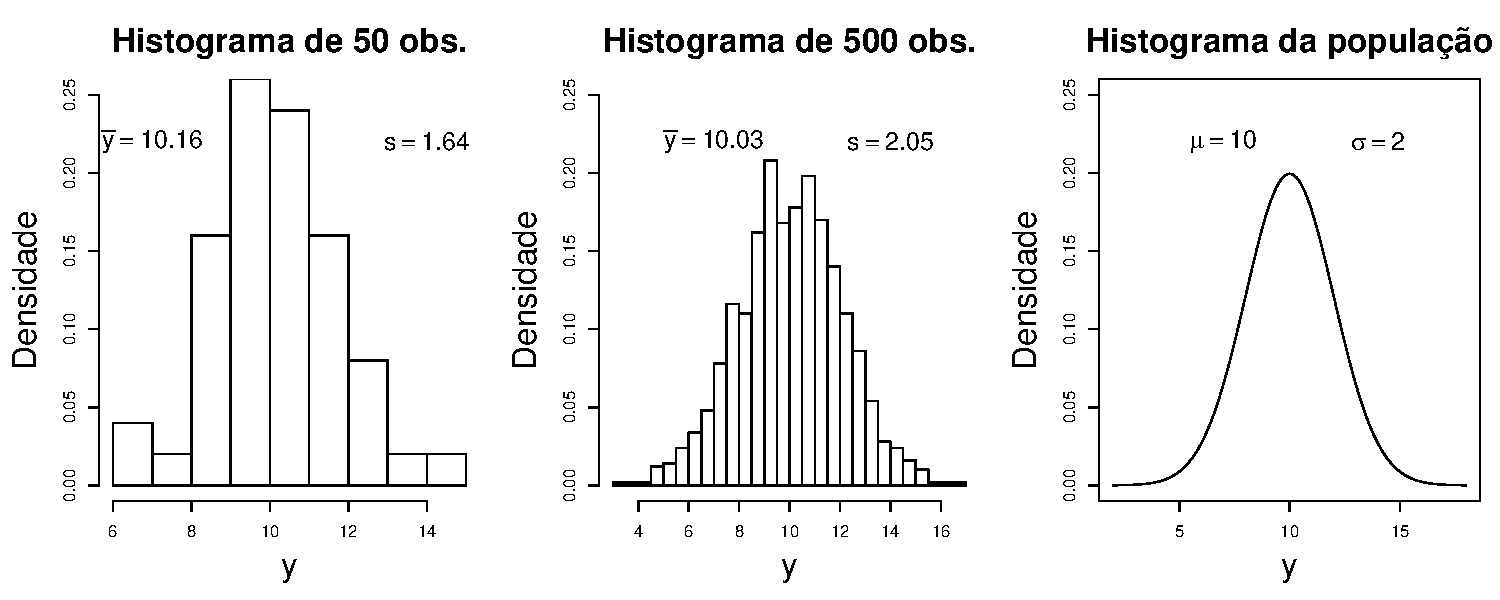
\includegraphics{probability_files/figure-latex/histToPop-1.pdf}

\begin{center}\rule{0.5\linewidth}{\linethickness}\end{center}

\subsubsection{Formatos das densidades}\label{formatos-das-densidades}

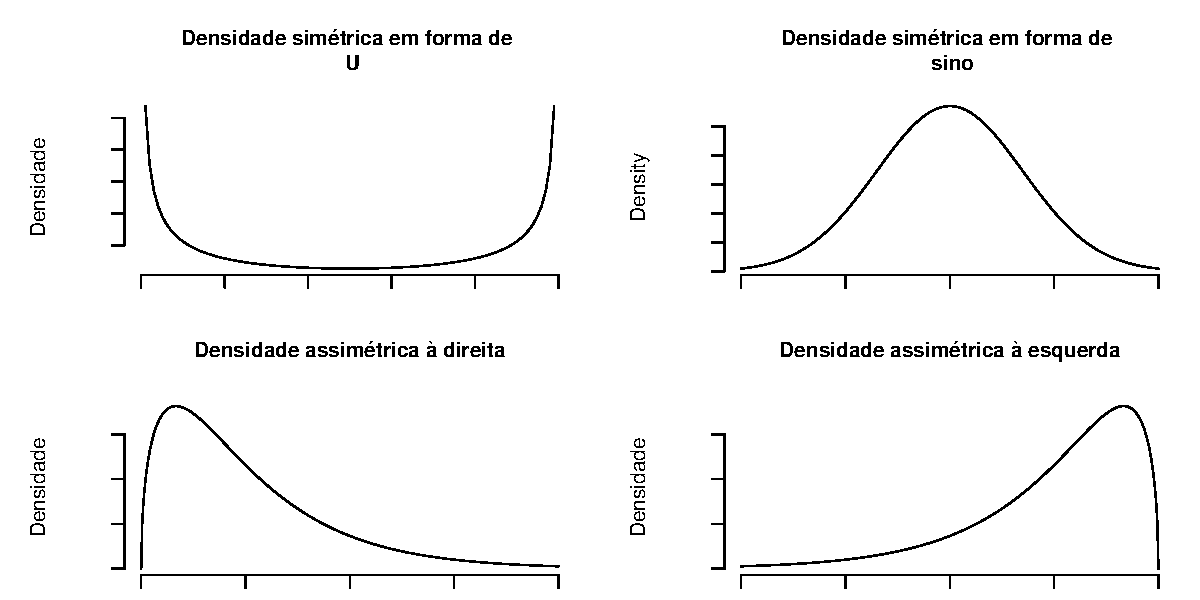
\includegraphics[width=\textwidth]{probability_files/figure-latex/densities-1}

\subsection{Distribuição Normal}\label{distribuicao-normal}

\begin{itemize}
\tightlist
\item
  A distribuição Normal é uma distribuição contínua determinada por 2
  parâmetros:

  \begin{itemize}
  \tightlist
  \item
    \(\mu\): a \textbf{média} (valor esperado), que determina onde a
    distribuição é centrada.
  \item
    \(\sigma^2\) a \textbf{variância}, que determina a dispersão da
    distribuição em torno da média.
  \end{itemize}
\item
  A distribuição tem uma função densidade de probabilidade em forma de
  sino:
  \[ f_Y(y;\mu,\sigma^2) = \frac{1}{\sqrt{2p\sigma^2}}\exp \left (-\frac{1}{2\sigma^2}(y-\mu)^2 \right ) \]
\item
  Quando uma variável aleatória \(Y\) segue uma distribuição normal com
  média \(\mu\) e variância \(\sigma^2\), então nós escrevemos que
  \(Y \sim \texttt{N}(\mu,\sigma^2)\).
\item
  Chamamos de distribuição \textbf{Normal padrão} uma distribuição
  Normal com média 0 e variância \(1\) e notamos isto por
  \(Z \sim \texttt{N}(0, 1)\).
\end{itemize}

\begin{center}\rule{0.5\linewidth}{\linethickness}\end{center}

\subsubsection{Alcance da distribuição
normal}\label{alcance-da-distribuicao-normal}

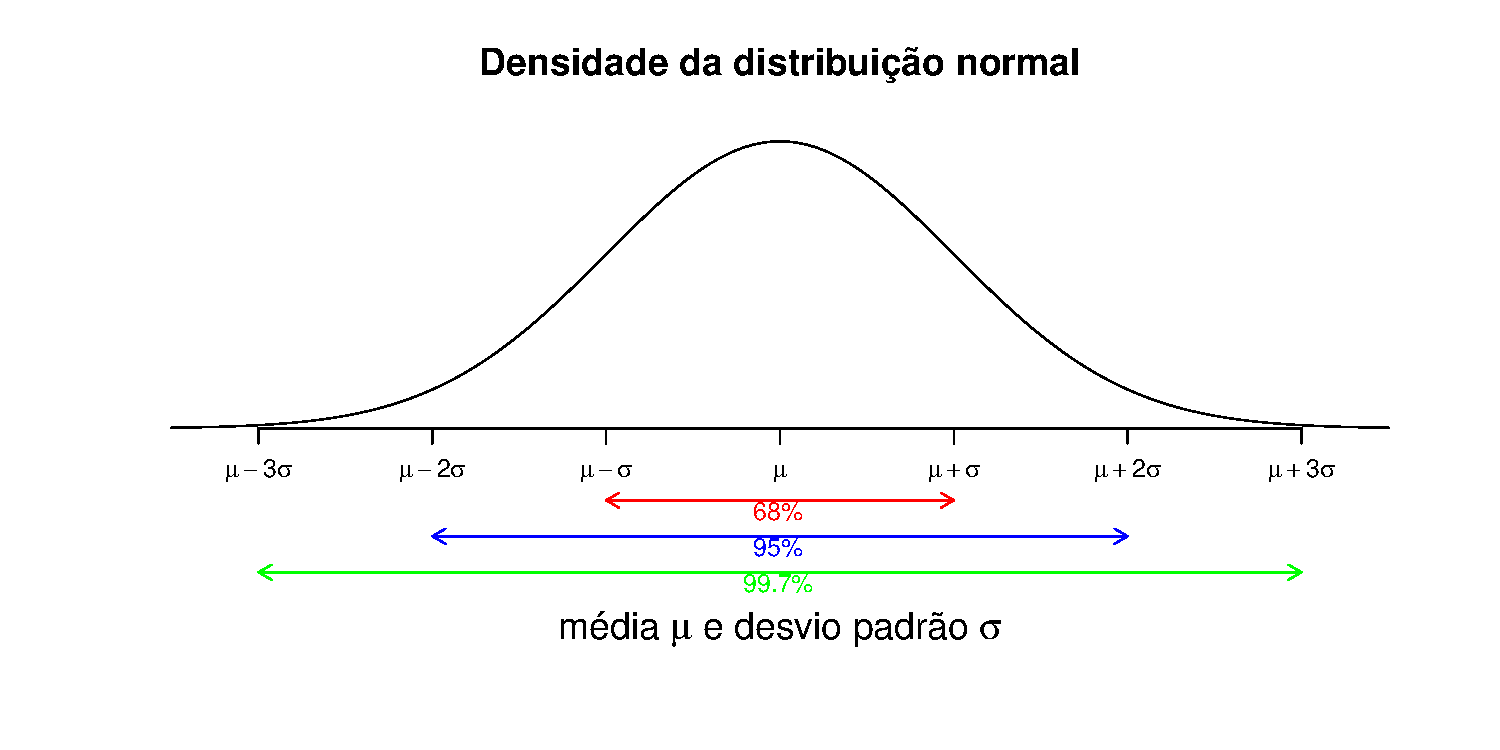
\includegraphics{probability_files/figure-latex/normalreach-1.pdf}

Interpretação:

\begin{itemize}
\tightlist
\item
  \(\approx\) 68\% da população está dentro de um desvio padrão da
  média.
\item
  \(\approx\) 95\% da população está dentro de 2 desvios padrão da
  média.
\item
  \(\approx\) 99.7\% da população está dentro de 3 desvios padrão da
  média.
\end{itemize}

\begin{center}\rule{0.5\linewidth}{\linethickness}\end{center}

\subsubsection{\texorpdfstring{Escore \(z\)}{Escore z}}\label{escore-z}

\begin{itemize}
\tightlist
\item
  Se \(Y\sim \texttt{N}(\mu,\sigma^2)\) então o escore-\(z\)
  correspondente é
  \[Z=\frac{Y-\mu}{\sigma}=\frac{\mathtt{observação-média}}{\mathtt{desvio\
    padrão}}\]
\item
  I.e. \(Z\) representa o número de desvios padrão da observação em
  relação à média.
\item
  \(Z\sim \texttt{N}(0,1)\), i.e. \(Z\) tem média zero e variância
  \(1\).
\item
  Isto implica que

  \begin{itemize}
  \tightlist
  \item
    \(Z\) situa-se entre \(-1\) e \(1\) com probabilidade de 0.6826
  \item
    \(Z\) situa-se entre \(-2\) e \(2\) com probabilidade de 0.9544
  \item
    \(Z\) situa-se entre \(-3\) e \(3\) com probabilidade de 0.9973
  \end{itemize}
\item
  Isto também implica que:

  \begin{itemize}
  \tightlist
  \item
    A probabilidade de \(Y\) estar entre \(\mu - z\sigma\) e
    \(\mu + z\sigma\) é igual a probabilidade de \(Z\) estar entre
    \(-z\) e \(z\).
  \end{itemize}
\end{itemize}

\begin{center}\rule{0.5\linewidth}{\linethickness}\end{center}

\subsubsection{Calculando probabilidades na distribuição normal
padrão}\label{calculando-probabilidades-na-distribuicao-normal-padrao}

\begin{itemize}
\tightlist
\item
  A função \texttt{pdist} produz a área à esquerda do valor \(z\)
  (quantil/percentil) que informamos (variável \texttt{q} na função),
  i.e.~mostra a probabilidade de obter um valor menor do que \(z\). O
  primeiro argumento de \texttt{pdist} denota a distribuição que estamos
  considerando.
\end{itemize}

\begin{Shaded}
\begin{Highlighting}[]
\CommentTok{#Para uma distribuição normal padrão, a probabilidade de obter um valor menor que 1 é:}
\NormalTok{left_prob <-}\StringTok{ }\KeywordTok{pdist}\NormalTok{(}\StringTok{"norm"}\NormalTok{, }\DataTypeTok{q =} \DecValTok{1}\NormalTok{, }\DataTypeTok{mean =} \DecValTok{0}\NormalTok{, }\DataTypeTok{sd =} \DecValTok{1}\NormalTok{)}
\end{Highlighting}
\end{Shaded}

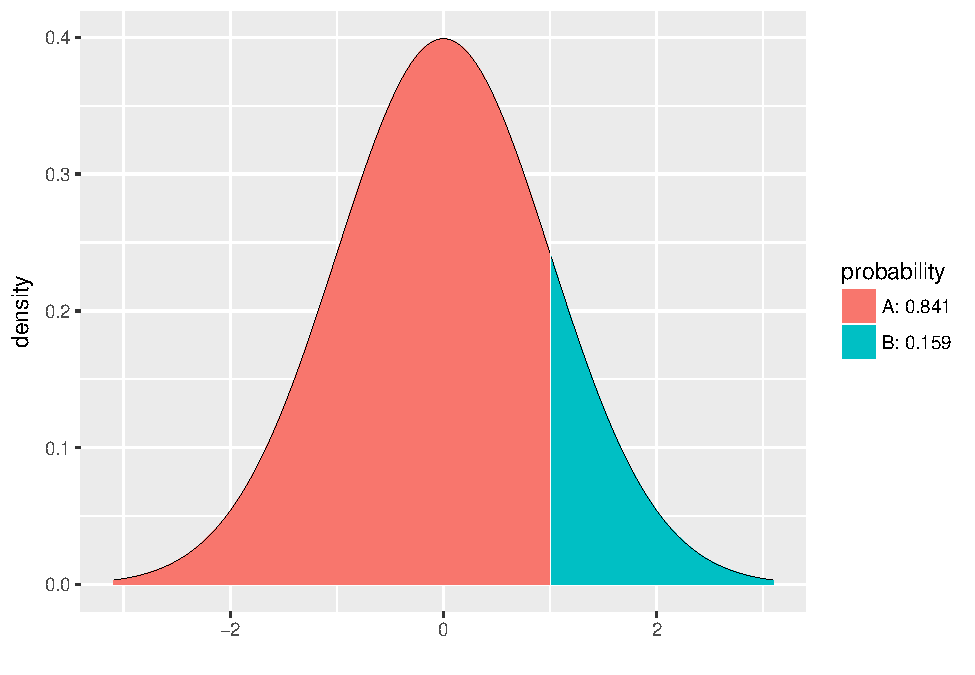
\includegraphics{probability_files/figure-latex/unnamed-chunk-12-1.pdf}

\begin{Shaded}
\begin{Highlighting}[]
\NormalTok{left_prob}
\end{Highlighting}
\end{Shaded}

\begin{verbatim}
## [1] 0.8413447
\end{verbatim}

\begin{Shaded}
\begin{Highlighting}[]
\NormalTok{right_prob <-}\StringTok{ }\DecValTok{1} \OperatorTok{-}\StringTok{ }\NormalTok{left_prob}
\NormalTok{right_prob}
\end{Highlighting}
\end{Shaded}

\begin{verbatim}
## [1] 0.1586553
\end{verbatim}

\begin{itemize}
\tightlist
\item
  Para \(z=1\) nós temos uma probabilidade à direita de \(p=0.1587\),
  então a probabilidade de uma observação entre \(-1\) e \(1\) é
  \(1 - 2 \cdot 0.1587 = 0.6826 = 68.26\%\) devido a simetria.
\end{itemize}

\begin{center}\rule{0.5\linewidth}{\linethickness}\end{center}

\subsubsection{Exemplo}\label{exemplo}

A escala de inteligência de Stanford-Binet é calibrada para ser
aproximadamente normal com média 100 e desvio padrão 16.

Qual é o 99-percentil dos escores de QI?

\begin{itemize}
\tightlist
\item
  O correpondente escore-\(z\) é \(Z=\frac{IQ-100}{16}\), o que
  significa que \(QI=16Z+100\).
\item
  O 99-percentil dos escores-\(z\) é 2.326 (pode ser calculado usando
  \texttt{qdist}).
\item
  Então, o 99-percentil dos escores de QI é: \[
    QI=16\cdot 2.326+100=137.2.
    \]
\item
  Então, esperamos que uma a cada cem pessoas tenha um QI superior a
  137.
\end{itemize}

\section{Distribuição da estatística
amostral}\label{distribuicao-da-estatistica-amostral}

\subsection{Estimativas e sua
variabilidade}\label{estimativas-e-sua-variabilidade}

Temos uma amostra \(y_1,y_2,\ldots,y_n\).

\begin{itemize}
\tightlist
\item
  A média amostral \(\bar{y}\) é a estimativa mais comum da média
  populacional \(\mu\).
\item
  O desvio padrão amostral, \(s\), é a estimativa mais comum do desvio
  padrão populacional \(\sigma\). Note que há uma incerteza (de amostra
  para amostra) conectada a estas estatísticas e, portanto, estamos
  interessados em descrever a sua \textbf{distribuição}.
\end{itemize}

\subsection{Distribuição da média
amostral}\label{distribuicao-da-media-amostral}

\begin{itemize}
\tightlist
\item
  Temos uma amostra \(y_1,y_2,\ldots,y_n\) de uma população com média
  \(\mu\) e desvio padrão \(\sigma\).
\item
  A média amostral \[\bar{y}=\frac{1}{n}(y_1+y_2+\ldots+y_n)\] tem
  distribuição

  \begin{itemize}
  \tightlist
  \item
    com média \(\mu\),
  \item
    e desvio padrão \(\frac{\sigma}{\sqrt{n}}\) (também chamado de
    \textbf{erro padrão}), e
  \item
    quando \(n\) cresce, a distribuição se aproxima de uma distribuição
    normal. Este resultado é provado usando o \textbf{teorema central do
    limite}.
  \end{itemize}
\end{itemize}

\begin{center}\rule{0.5\linewidth}{\linethickness}\end{center}

\subsubsection{Teorema Central do
Limite}\label{teorema-central-do-limite}

\begin{itemize}
\tightlist
\item
  Os pontos anteriores podem ser resumidos por \[
    \bar{y}\sim \texttt{N}\bigg(\mu,\frac{\sigma^{2}}{{n}}\bigg),
    \] i.e. \(\bar{y}\) tem distribuição aproximadamente normal com
  média \(\mu\) e erro padrão \(\frac{\sigma}{\sqrt{n}}\).
\item
  Quando a amostra é suficientemente grande (para que a aproximação seja
  boa) isto nos permite fazer as seguintes observações:

  \begin{itemize}
  \tightlist
  \item
    Nós estamos \(95\%\) certos de que \(\bar{y}\) está no intervalo de
    \(\mu-2\frac{\sigma}{\sqrt{n}}\) a \(\mu+2\frac{\sigma}{\sqrt{n}}\).
  \item
    Estamos quase completamente certos de que \(\bar{y}\) está no
    intervalo \(\mu-3\frac{\sigma}{\sqrt{n}}\) a
    \(\mu+3\frac{\sigma}{\sqrt{n}}\).
  \end{itemize}
\end{itemize}

\subsubsection{Ilustração do TCL}\label{ilustracao-do-tcl}

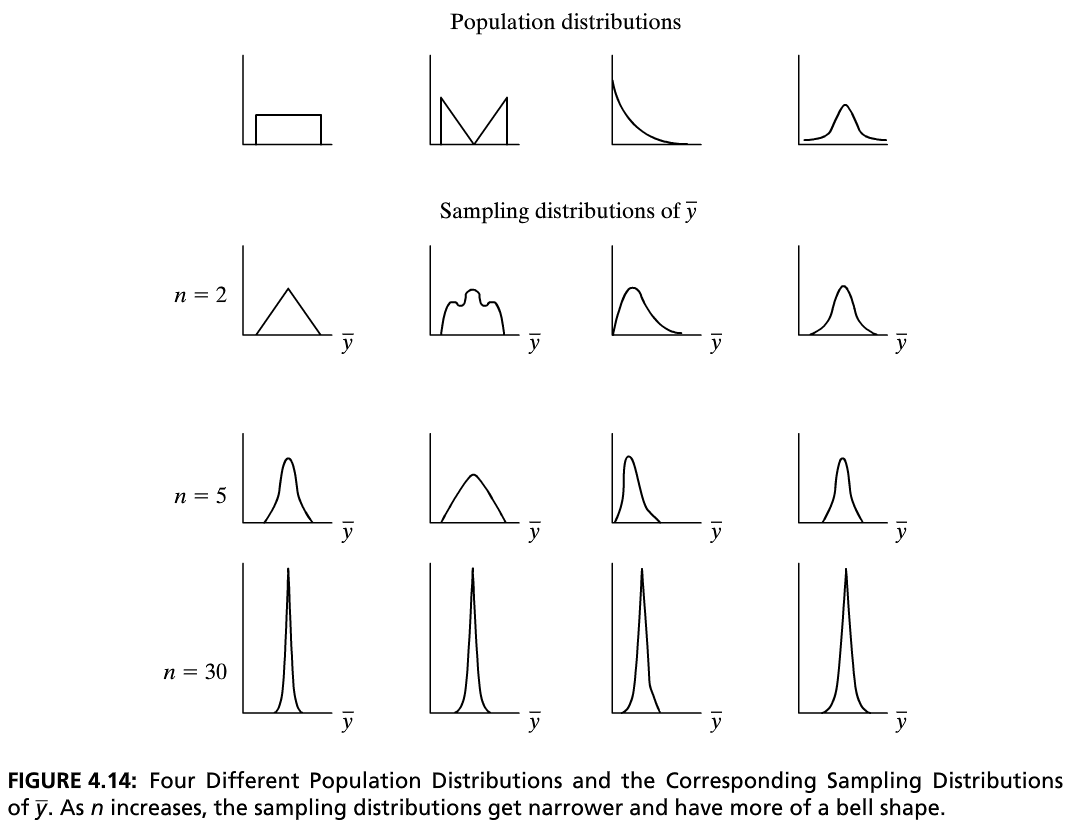
\includegraphics{C:/Users/fsabino/Desktop/Codes/papers/Introductory_Stat_I/notebook/AgrestiCLT.png}

\begin{center}\rule{0.5\linewidth}{\linethickness}\end{center}

\subsubsection{Exemplo}\label{exemplo-1}

\begin{itemize}
\tightlist
\item
  Índice de Massa Corporal (IMC) de pessoas do norte da europa (2010)
  tem média \(\mu=25.8\) kg/\(\mathtt{m}^2\) e desvio padrão \(4.8\)
  kg/\(\mathtt{m}^2\).
\item
  Uma amostra aleatória de \(n=100\) clientes de uma hamburgueria teve
  um IMC médio dado por \(\bar{y}=27.2\).
\item
  Se comer hamburguer ``não influencia'' o IMC (e a amostra é
  representativa da população de interesse), então
  \[\bar{y} \approx \texttt{N}\bigg(\mu,\frac{\sigma^2}{n}\bigg)=\texttt{N}(25.8,0.48^2).\]
\item
  Para amostra o escore-\(z\) observado
  \[z_{obs}=\frac{27.2-25.8}{0.48}=2.92\]
\item
  Lembrando que o escore-\(z\) é (aproximadamente) normal padrão, a
  probabilidade de obter uma pontuação mais alta que o escore-\(z\) é:
\end{itemize}

\begin{Shaded}
\begin{Highlighting}[]
\DecValTok{1} \OperatorTok{-}\StringTok{ }\KeywordTok{pdist}\NormalTok{(}\StringTok{"norm"}\NormalTok{, }\DataTypeTok{mean =} \DecValTok{0}\NormalTok{, }\DataTypeTok{sd =} \DecValTok{1}\NormalTok{, }\DataTypeTok{q =} \FloatTok{2.92}\NormalTok{, }\DataTypeTok{xlim =} \KeywordTok{c}\NormalTok{(}\OperatorTok{-}\DecValTok{4}\NormalTok{, }\DecValTok{4}\NormalTok{))}
\end{Highlighting}
\end{Shaded}

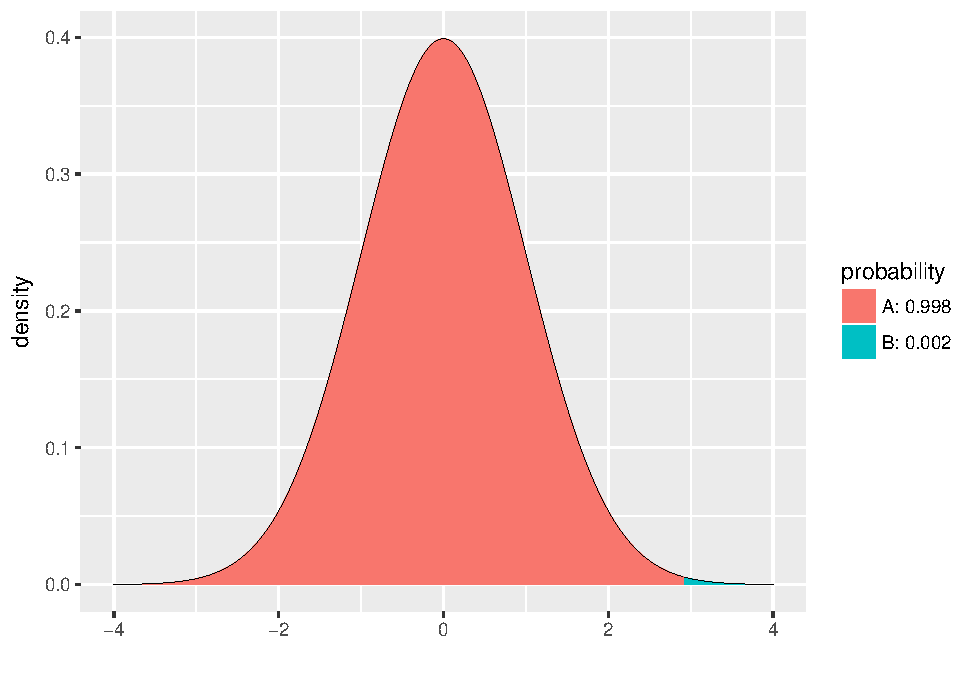
\includegraphics{probability_files/figure-latex/unnamed-chunk-14-1.pdf}

\begin{verbatim}
## [1] 0.001750157
\end{verbatim}

\begin{itemize}
\tightlist
\item
  Assim, é altamente imporvável obter uma amostra aleatória com um
  escore-\(z\) tão alto. Há evidências de que os clientes da
  hamburgueira tem um IMC médio maior que a média populacional.
\end{itemize}


\end{document}
